\documentclass{csbeamer}

\usepackage{dsfont}
\usepackage{amsmath}
\usepackage{amssymb}
\usepackage{algorithm}
\usepackage{algpseudocode}
\usepackage{bm}

% Add custom color definitions for Deep RL
\definecolor{drlmain}{HTML}{6A1B9A}
\definecolor{drlaccent}{HTML}{FF6B35}
\definecolor{drllight}{HTML}{9C27B0}
\definecolor{drlsecondary}{HTML}{00897B}
\definecolor{drlpolicy}{HTML}{D32F2F}
\definecolor{drlvalue}{HTML}{1976D2}
\definecolor{drlactor}{HTML}{E91E63}
\definecolor{drlcritic}{HTML}{3F51B5}
\definecolor{drlgradient}{HTML}{FF9800}
\definecolor{drladvantage}{HTML}{4CAF50}
\definecolor{drlneural}{HTML}{7B1FA2}

\university{St. Francis Xavier University}
\department{Department of Computer Science}
\course{CSCI-531 - Reinforcement Learning}
\courseshort{CSCI-531 - RL}
\term{Fall 2025}
\author{Dr. Jean-Alexis Delamer}

\title{Deep Reinforcement Learning:\\ Policy Gradient Methods}

\begin{document}

\frame{\titlepage}

% Section: Introduction
\section{Introduction}

\subsection{From Tabular to Deep RL}

\begin{frame}
    \frametitle{The Journey So Far}

    \begin{block}<1->{What We've Learned}
        \begin{itemize}
            \item<1-> \textcolor{drlmain}{\textbf{Monte Carlo}}: Learning from complete episodes
            \item<2-> \textcolor{drlsecondary}{\textbf{TD Learning}}: Bootstrapping from partial trajectories
            \item<3-> \textcolor{drlvalue}{\textbf{Policy Approximation}}: Parameterized policies (without neural networks)
        \end{itemize}
    \end{block}

    \begin{block}<4->{The Limitation}
        \begin{center}
            \textcolor{drlaccent}{\large \textbf{What if the state space is enormous or continuous?}}
        \end{center}
        \begin{itemize}
            \item<5-> Can't store a value for every state
            \item<6-> Can't store a policy for every state-action pair
            \item<7-> Need to \textcolor{drlneural}{\textbf{generalize}} across states
        \end{itemize}
    \end{block}
\end{frame}

\begin{frame}
    \frametitle{Real-World Challenges}

    \begin{block}<1->{Consider These Problems...}
        \begin{itemize}
            \item<1-> \textbf{Atari Games}: $210 \times 160$ pixels $\times$ 3 colors = $256^{100,800}$ states
            \item<2-> \textbf{Robot Control}: Continuous joint angles, velocities, forces
            \item<3-> \textbf{Go}: $3^{361} \approx 10^{172}$ possible board positions
            \item<4-> \textbf{Self-Driving Cars}: Camera images, sensor readings, traffic patterns
        \end{itemize}
    \end{block}

    \begin{block}<5->{The Deep Learning Solution}
        \begin{center}
            \textcolor{drlneural}{\Large \textbf{Use neural networks as function approximators!}}
        \end{center}
        \begin{itemize}
            \item<6-> Learn patterns and features automatically
            \item<7-> Generalize to unseen states
            \item<8-> Handle high-dimensional inputs
        \end{itemize}
    \end{block}
\end{frame}

\begin{frame}
    \frametitle{Deep Reinforcement Learning}

    \begin{center}
        \begin{tikzpicture}[scale=0.9]
            % Traditional RL
            \node[rectangle, draw=drlmain, fill=drlmain!20, rounded corners=4pt, minimum width=3cm, minimum height=1cm] (trad) at (0,3)
                {\textbf{Traditional RL}};
            \node[below=3pt of trad] {Tables, Linear Functions};

            % Deep Learning
            \node[rectangle, draw=drlneural, fill=drlneural!20, rounded corners=4pt, minimum width=3cm, minimum height=1cm] (dl) at (0,0)
                {\textbf{Deep Learning}};
            \node[below=3pt of dl] {Neural Networks};

            % Deep RL
            \node[rectangle, draw=drlaccent, fill=drlaccent!20, rounded corners=8pt, thick, minimum width=4cm, minimum height=1.5cm] (drl) at (6,1.5)
                {\Large \textbf{Deep RL}};
            \node[below=3pt of drl] {Best of Both Worlds};

            % Arrows
            \draw[->, very thick, drlmain] (trad.east) -- (drl.west);
            \draw[->, very thick, drlneural] (dl.east) -- (drl.west);
        \end{tikzpicture}
    \end{center}

    \vspace{1em}

    \begin{block}<2->{Key Insight}
        \textcolor{drlaccent}{\textbf{Combine RL algorithms with neural network function approximation}}
    \end{block}
\end{frame}

\subsection{From Approximation to Deep RL}

\begin{frame}
    \frametitle{Recall: Policy Approximation (Linear Methods)}

    \begin{block}<1->{What You've Learned}
        Policy approximation with \textcolor{drlmain}{\textbf{linear function approximation}}:
        \begin{itemize}
            \item<2-> Features: $\mathbf{x}(s)$ are hand-crafted
            \item<3-> Parameters: $w$ is a weight vector
        \end{itemize}
    \end{block}

    \begin{block}<4->{The Limitation}
        \begin{itemize}
            \item<5-> \textcolor{drlaccent}{\textbf{Manual feature engineering}}: Need to design $\mathbf{x}(s)$
            \item<6-> \textcolor{drlaccent}{\textbf{Limited expressiveness}}: Linear combinations only
            \item<7-> \textcolor{drlaccent}{\textbf{Doesn't scale}}: Complex problems need complex features
        \end{itemize}
    \end{block}
\end{frame}

\begin{frame}
    \frametitle{The Shift to Deep Learning}

    \begin{block}<1->{Deep RL = Replace Linear with Neural Networks}
        \begin{center}
            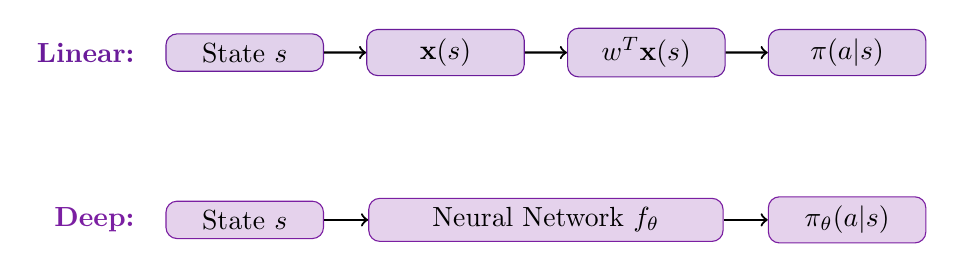
\begin{tikzpicture}[scale=0.85]
                % Linear approximation
                \node[rectangle, draw=drlmain, fill=drlmain!20, rounded corners=4pt, minimum width=2cm] (state1) at (0,3)
                    {State $s$};
                \node[rectangle, draw=drlmain, fill=drlmain!20, rounded corners=4pt, minimum width=2cm] (features) at (3,3)
                    {$\mathbf{x}(s)$};
                \node[rectangle, draw=drlmain, fill=drlmain!20, rounded corners=4pt, minimum width=2cm] (linear) at (6,3)
                    {$w^T \mathbf{x}(s)$};
                \node[rectangle, draw=drlmain, fill=drlmain!20, rounded corners=4pt, minimum width=2cm] (output1) at (9,3)
                    {$\pi(a|s)$};

                \draw[->, thick] (state1) -- (features);
                \draw[->, thick] (features) -- (linear);
                \draw[->, thick] (linear) -- (output1);

                \node[left] at (-1.5,3) {\textcolor{drlmain}{\textbf{Linear:}}};

                % Neural network
                \node[rectangle, draw=drlneural, fill=drlneural!20, rounded corners=4pt, minimum width=2cm] (state2) at (0,0.5)
                    {State $s$};
                \node[rectangle, draw=drlneural, fill=drlneural!20, rounded corners=4pt, minimum width=4.5cm] (nn) at (4.5,0.5)
                    {Neural Network $f_\theta$};
                \node[rectangle, draw=drlneural, fill=drlneural!20, rounded corners=4pt, minimum width=2cm] (output2) at (9,0.5)
                    {$\pi_\theta(a|s)$};

                \draw[->, thick] (state2) -- (nn);
                \draw[->, thick] (nn) -- (output2);

                \node[left] at (-1.5,0.5) {\textcolor{drlneural}{\textbf{Deep:}}};
            \end{tikzpicture}
        \end{center}
    \end{block}

    \begin{block}<2->{Key Difference}
        \textcolor{drlneural}{\textbf{Neural networks learn features automatically!}} \\
        No need to hand-craft $\mathbf{x}(s)$.
    \end{block}
\end{frame}

\begin{frame}
    \frametitle{Notation Changes: Linear vs Deep}

    \begin{block}<1->{Linear Approximation (What You Know)}
        \begin{itemize}
            \item<2-> Parameters: $w \in \mathbb{R}^d$ (weight vector)
            \item<3-> Features: $x(s)$ explicitly written
            \item<4-> Update: Based on feature vectors
        \end{itemize}
    \end{block}

    \begin{block}<5->{Deep RL (New Notation)}
        \begin{itemize}
            \item<6-> Parameters: $\theta$ (all neural network weights and biases)
            \item<7-> Policy: $\pi_\theta(a|s)$ (\textcolor{drlaccent}{subscript $\theta$} emphasizes parameterization)
            \item<8-> Features: \textcolor{drlneural}{\textbf{Learned automatically}} by hidden layers
            \item<9-> Update: Using backpropagation through the network
        \end{itemize}
    \end{block}

    \begin{block}<11->{Why the Subscript?}
        $\pi_\theta$ emphasizes that we're optimizing over a \textcolor{drlneural}{\textbf{family of policies}} parameterized by $\theta$
    \end{block}
\end{frame}

\begin{frame}
    \frametitle{Optimization: Minimization vs Maximization}

    \begin{columns}
        \begin{column}{0.5\textwidth}
            \begin{block}<1->{Value Approximation}
                \textcolor{drlvalue}{\textbf{Minimize Error}}
                \begin{align*}
                    \text{Loss: } L(\theta) &= (v_\pi(s) - \hat{v}(s,\theta))^2 \\
                    \theta &\leftarrow \theta - \alpha \nabla_\theta L
                \end{align*}
                \begin{itemize}
                    \item<3-> \textcolor{drlaccent}{Gradient \textbf{descent}}
                    \item<4-> Minimize prediction error
                \end{itemize}
            \end{block}
        \end{column}
        \begin{column}{0.5\textwidth}
            \begin{block}<5->{Policy Gradient}
                \textcolor{drlpolicy}{\textbf{Maximize Return}}
                \begin{align*}
                    \text{Objective: } J(\theta) &= \mathbb{E}[G_t] \\
                    \theta &\leftarrow \theta + \alpha \nabla_\theta J
                \end{align*}
                \begin{itemize}
                    \item<7-> \textcolor{drladvantage}{Gradient \textbf{ascent}}
                    \item<8-> Maximize expected reward
                \end{itemize}
            \end{block}
        \end{column}
    \end{columns}
    \begin{block}<9->{Key Distinction}
        \begin{itemize}
            \item<10-> \textcolor{drlvalue}{\textbf{Value methods}}: Fit to targets $\rightarrow$ minimize loss
            \item<11-> \textcolor{drlpolicy}{\textbf{Policy methods}}: Optimize performance $\rightarrow$ maximize return
        \end{itemize}
    \end{block}
\end{frame}

\begin{frame}
    \frametitle{Same Idea, Different Framework}

    \begin{block}<1->{Common Thread}
        Both use \textcolor{drlmain}{\textbf{gradient-based optimization}} to update parameters!
    \end{block}

    \begin{center}
        \begin{tikzpicture}[scale=0.8]
            % Value approximation
            \node[rectangle, draw=drlvalue, fill=drlvalue!20, rounded corners=4pt, minimum width=3cm, text width=2.8cm, align=center] (val) at (0,2)
                {\textbf{Value Approx.} \\ Minimize $L(\theta)$};
            \node[below=5pt of val] {\small $\downarrow$ error};

            % Policy gradient
            \node[rectangle, draw=drlpolicy, fill=drlpolicy!20, rounded corners=4pt, minimum width=3cm, text width=2.8cm, align=center] (pol) at (6,2)
                {\textbf{Policy Gradient} \\ Maximize $J(\theta)$};
            \node[below=5pt of pol] {\small $\uparrow$ reward};

            % Common ground
            \node[rectangle, draw=drlneural, fill=drlneural!20, rounded corners=6pt, thick, minimum width=4cm, text width=3.8cm, align=center] (common) at (3,-1)
                {\textbf{Both use} \\ $\theta \leftarrow \theta \pm \alpha \nabla_\theta \text{(objective)}$};

            \draw[->, very thick, drlvalue] (val.south) -- (common.north west);
            \draw[->, very thick, drlpolicy] (pol.south) -- (common.north east);
        \end{tikzpicture}
    \end{center}

    \begin{block}<2->{Today's Focus}
        We'll focus on \textcolor{drlpolicy}{\textbf{policy gradient methods}} where we directly optimize the policy to maximize return.
    \end{block}
\end{frame}

\subsection{Two Approaches to RL}

\begin{frame}
    \frametitle{Value-Based vs Policy-Based Methods}

    \begin{columns}
        \begin{column}{0.5\textwidth}
            \begin{block}<1->{Value-Based Methods}
                \begin{center}
                    \textcolor{drlvalue}{\textbf{Learn Value Function}}
                \end{center}
                \begin{itemize}
                    \item<2-> Learn $V(s)$ or $Q(s,a)$
                    \item<3-> Policy is \textcolor{drlvalue}{\textbf{implicit}}
                    \item<4-> Extract policy: $\pi(s) = \arg\max_a Q(s,a)$
                    \item<5-> Examples: Q-Learning, DQN
                \end{itemize}
            \end{block}
        \end{column}
        \begin{column}{0.5\textwidth}
            \begin{block}<6->{Policy-Based Methods}
                \begin{center}
                    \textcolor{drlpolicy}{\textbf{Learn Policy Directly}}
                \end{center}
                \begin{itemize}
                    \item<7-> Learn $\pi_\theta(a|s)$ directly
                    \item<8-> Policy is \textcolor{drlpolicy}{\textbf{explicit}}
                    \item<9-> No need for value function
                    \item<10-> Examples: REINFORCE, PPO
                \end{itemize}
            \end{block}
        \end{column}
    \end{columns}

    \vspace{1em}

    \begin{block}<11->{Today's Focus}
        \textcolor{drlaccent}{\textbf{Policy-Based Methods}} (and later, combining both!)
    \end{block}
\end{frame}

\begin{frame}
    \frametitle{Why Learn Policies Directly?}

    \begin{block}<1->{Advantages of Policy-Based Methods}
        \begin{enumerate}
            \item<2-> \textcolor{drlpolicy}{\textbf{Better Convergence}}: Smoother optimization landscape
            \item<3-> \textcolor{drlpolicy}{\textbf{Effective in High Dimensions}}: Natural for large action spaces
            \item<4-> \textcolor{drlpolicy}{\textbf{Stochastic Policies}}: Can learn probabilistic behavior
            \item<5-> \textcolor{drlpolicy}{\textbf{Continuous Actions}}: Natural for robot control
        \end{enumerate}
    \end{block}

    \begin{block}<6->{Example: Rock-Paper-Scissors}
        \begin{itemize}
            \item<7-> \textbf{Optimal policy}: Play each action with probability $\frac{1}{3}$
            \item<8-> \textcolor{drlvalue}{\textbf{Value-based}}: All actions have same value, hard to represent stochastic policy
            \item<9-> \textcolor{drlpolicy}{\textbf{Policy-based}}: Directly output probabilities $[0.33, 0.33, 0.33]$
        \end{itemize}
    \end{block}
\end{frame}

% Section: Policy Gradient Theorem
\section{Policy Gradient Methods}

\subsection{The Policy Gradient Objective}

\begin{frame}
    \frametitle{What Are We Trying to Optimize?}

    \begin{block}<1->{The Goal}
        Find policy parameters $\theta$ that maximize expected return:
        \begin{equation*}
            J(\theta) = \mathbb{E}_{\tau \sim \pi_\theta} \left[ G_0 \right] = \mathbb{E}_{\tau \sim \pi_\theta} \left[ \sum_{t=0}^T \gamma^t r_t \right]
        \end{equation*}
        where $\tau$ is a trajectory: $s_0, a_0, r_0, s_1, a_1, r_1, \ldots$
    \end{block}

    \begin{block}<2->{Notation}
        \begin{itemize}
            \item<2-> $\pi_\theta(a|s)$: Policy parameterized by $\theta$ (neural network weights)
            \item<3-> $J(\theta)$: Performance objective (total expected reward)
            \item<4-> $\gamma$: Discount factor
        \end{itemize}
    \end{block}

    \only<5->{
        \textcolor{drlaccent}{\textbf{How do we adjust $\theta$ to increase $J(\theta)$?}}
    }
\end{frame}

\begin{frame}
    \frametitle{Gradient Ascent on the Policy}

    \begin{block}<1->{The Optimization Approach}
        Use gradient ascent to maximize $J(\theta)$: $\theta_{t+1} = \theta_t + \alpha \nabla_\theta J(\theta)$
    \end{block}

    \begin{center}
        \begin{tikzpicture}[scale=0.8]
            % Draw a curved surface representing J(theta)
            \draw[thick, drlmain] plot[smooth, domain=-2:2] (\x, {-0.3*(\x-0.5)*(\x-0.5) + 2.5});

            % Draw gradient arrows
            \only<2->{
                \draw[->, very thick, drlgradient] (-1.5, 1.88) -- (-1.2, 2.23);
                \node[below] at (-1.5, 1.88) {$\theta_t$};
            }

            \only<3->{
                \draw[->, very thick, drlgradient] (-0.5, 2.47) -- (-0.2, 2.52);
                \node[below] at (-0.5, 2.47) {$\theta_{t+1}$};
            }

            \only<4->{
                \draw[->, very thick, drlgradient] (0.5, 2.53) -- (0.6, 2.53);
                \node[above] at (0.5, 2.53) {$\theta^*$};

            }
            \only<5->{
                \node at (0.5, 3) {\textcolor{drlaccent}{Optimal!}};
            }

            % Axes
            \draw[->] (-2.5,0) -- (2.5,0) node[right] {$\theta$};
            \draw[->] (-2.5,0) -- (-2.5,3) node[above] {$J(\theta)$};
        \end{tikzpicture}
    \end{center}

    \begin{block}<5->{Challenge}
        How do we compute $\nabla_\theta J(\theta)$ when $J$ depends on environment dynamics?
    \end{block}
\end{frame}

\subsection{The Policy Gradient Theorem}

\begin{frame}
    \frametitle{Deriving the Policy Gradient: The Challenge}

    \begin{block}<1->{What We Want}
        Compute $\nabla_\theta J(\theta)$ where:
        \begin{equation*}
            J(\theta) = \mathbb{E}_{\tau \sim \pi_\theta} [G_0]
        \end{equation*}
    \end{block}

    \begin{block}<2->{The Problem}
        \begin{itemize}
            \item<3-> Expected value is over \textcolor{drlaccent}{\textbf{trajectories}} $\tau$
            \item<4-> Trajectory distribution depends on:
                \begin{itemize}
                    \item Policy $\pi_\theta$ (which we control)
                    \item Environment dynamics $p(s'|s,a)$ (which we \textcolor{drlaccent}{\textbf{don't know}}!)
                \end{itemize}
            \item<5-> Can't directly differentiate through unknown environment!
        \end{itemize}
    \end{block}

    \begin{block}<6->{The Question}
        \textcolor{drlmain}{\textbf{How do we take gradient w.r.t. $\theta$ when expectation involves unknown dynamics?}}
    \end{block}
\end{frame}

\begin{frame}
    \frametitle{Step 1: Trajectory Probability}

    \begin{block}<1->{Breaking Down a Trajectory}
        A trajectory $\tau = (s_0, a_0, r_0, s_1, a_1, r_1, \ldots, s_T)$ has probability:
        \begin{equation*}
            P(\tau|\theta) = p(s_0) \prod_{t=0}^{T-1} \pi_\theta(a_t|s_t) p(s_{t+1}|s_t, a_t)
        \end{equation*}
    \end{block}

    \begin{block}<2->{Components}
        \begin{itemize}
            \item<3-> \textcolor{drlmain}{$p(s_0)$}: Initial state distribution (given by environment)
            \item<4-> \textcolor{drlpolicy}{$\pi_\theta(a_t|s_t)$}: Policy (depends on $\theta$)
            \item<5-> \textcolor{drlaccent}{$p(s_{t+1}|s_t, a_t)$}: Transition dynamics (unknown!)
        \end{itemize}
    \end{block}
\end{frame}

\begin{frame}
    \frametitle{Step 1: Trajectory Probability}

    \begin{block}{Breaking Down a Trajectory}
        A trajectory $\tau = (s_0, a_0, r_0, s_1, a_1, r_1, \ldots, s_T)$ has probability:
        \begin{equation*}
            P(\tau|\theta) = p(s_0) \prod_{t=0}^{T-1} \pi_\theta(a_t|s_t) p(s_{t+1}|s_t, a_t)
        \end{equation*}
    \end{block}

    \begin{block}<2->{Objective as Expectation}
        \begin{equation*}
            J(\theta) = \mathbb{E}_{\tau \sim P(\tau|\theta)} [G(\tau)] = \int_\tau P(\tau|\theta) G(\tau) d\tau
        \end{equation*}
        where $G(\tau) = \sum_{t=0}^T \gamma^t r_t$ is the return of trajectory $\tau$.
    \end{block}
\end{frame}

\begin{frame}
    \frametitle{Step 2: The Log Derivative Trick}

    \begin{block}<1->{Taking the Gradient}
        \begin{equation*}
            \nabla_\theta J(\theta) = \nabla_\theta \int_\tau P(\tau|\theta) G(\tau) d\tau \onslide<2->{= \int_\tau \nabla_\theta P(\tau|\theta) G(\tau) d\tau}
        \end{equation*}
    \end{block}

    \begin{block}<3->{The Trick: Multiply and Divide by $P(\tau|\theta)$}
        \begin{align*}
            \nabla_\theta J(\theta) &= \int_\tau \frac{P(\tau|\theta)}{P(\tau|\theta)} \nabla_\theta P(\tau|\theta) G(\tau) d\tau \\
            \onslide<4->{&= \int_\tau P(\tau|\theta) \frac{\nabla_\theta P(\tau|\theta)}{P(\tau|\theta)} G(\tau) d\tau}
        \end{align*}
    \end{block}
\end{frame}

\begin{frame}
    \frametitle{Step 2: The Log Derivative Trick}

    \begin{block}{Taking the Gradient}
        \begin{equation*}
            \nabla_\theta J(\theta) = \nabla_\theta \int_\tau P(\tau|\theta) G(\tau) d\tau = \int_\tau \nabla_\theta P(\tau|\theta) G(\tau) d\tau
        \end{equation*}
        \begin{equation*}
            \nabla_\theta J(\theta) = \int_\tau P(\tau|\theta) \frac{\nabla_\theta P(\tau|\theta)}{P(\tau|\theta)} G(\tau) d\tau
        \end{equation*}
    \end{block}

    \begin{block}<2->{Using the Log Derivative Identity}
        Recall: $\nabla_\theta \log f(\theta) = \frac{\nabla_\theta f(\theta)}{f(\theta)}$
        \begin{equation*}
            \nabla_\theta J(\theta) = \int_\tau P(\tau|\theta) \nabla_\theta \log P(\tau|\theta) G(\tau) d\tau
        \end{equation*}
    \end{block}
\end{frame}

\begin{frame}
    \frametitle{Step 3: Simplifying the Log Probability}

    \begin{block}<1->{Log of the Trajectory Probability}
        \begin{align*}
            \log P(\tau|\theta) &= \log \left[ p(s_0) \prod_{t=0}^{T-1} \pi_\theta(a_t|s_t) p(s_{t+1}|s_t, a_t) \right] \\
            \onslide<2->{&= \log p(s_0) + \sum_{t=0}^{T-1} \log \pi_\theta(a_t|s_t) + \sum_{t=0}^{T-1} \log p(s_{t+1}|s_t, a_t)}
        \end{align*}
    \end{block}
\end{frame}

\begin{frame}
    \frametitle{Step 3: Simplifying the Log Probability}

    \begin{block}{Log of the Trajectory Probability}
        $\log P(\tau|\theta) = \log p(s_0) + \sum_{t=0}^{T-1} \log \pi_\theta(a_t|s_t) + \sum_{t=0}^{T-1} \log p(s_{t+1}|s_t, a_t)$
    \end{block}
    \begin{block}{Taking the Gradient w.r.t. $\theta$}
        $\nabla_\theta \log P(\tau|\theta) = \nabla_\theta \log p(s_0) + \sum_{t=0}^{T-1} \nabla_\theta \log \pi_\theta(a_t|s_t) + \sum_{t=0}^{T-1} \nabla_\theta \log p(s_{t+1}|s_t, a_t)$
    \end{block}
    \begin{block}<2->{The Magic: Terms Vanish!}
        \begin{itemize}
            \item<3-> \textcolor{drladvantage}{$\nabla_\theta \log p(s_0) = 0$} (initial state doesn't depend on $\theta$)
            \item<4-> \textcolor{drladvantage}{$\nabla_\theta \log p(s_{t+1}|s_t, a_t) = 0$} (dynamics don't depend on $\theta$)
        \end{itemize}
    \end{block}
\end{frame}

\begin{frame}
    \frametitle{Step 4: The Beautiful Result}

    \begin{block}<1->{Only Policy Terms Remain!}
        \begin{equation*}
            \nabla_\theta \log P(\tau|\theta) = \sum_{t=0}^{T-1} \nabla_\theta \log \pi_\theta(a_t|s_t)
        \end{equation*}
    \end{block}

    \begin{block}<2->{Substituting Back}
        \begin{align*}
            \nabla_\theta J(\theta) &= \int_\tau P(\tau|\theta) \nabla_\theta \log P(\tau|\theta) G(\tau) d\tau \\
            \onslide<3->{&= \int_\tau P(\tau|\theta) \left[ \sum_{t=0}^{T-1} \nabla_\theta \log \pi_\theta(a_t|s_t) \right] G(\tau) d\tau \\}
        \end{align*}
    \end{block}
\end{frame}

\begin{frame}
    \frametitle{Step 4: The Beautiful Result}

    \begin{block}{Only Policy Terms Remain!}
        \begin{equation*}
            \nabla_\theta \log P(\tau|\theta) = \sum_{t=0}^{T-1} \nabla_\theta \log \pi_\theta(a_t|s_t)
        \end{equation*}
    \end{block}

    \begin{block}{Substituting Back}
        \begin{align*}
            \nabla_\theta J(\theta) &= \int_\tau P(\tau|\theta) \nabla_\theta \log P(\tau|\theta) G(\tau) d\tau = \int_\tau P(\tau|\theta) \left[ \sum_{t=0}^{T-1} \nabla_\theta \log \pi_\theta(a_t|s_t) \right] G(\tau) d\tau \\
            \onslide<2->{&= \mathbb{E}_{\tau \sim \pi_\theta} \left[ \sum_{t=0}^{T-1} \nabla_\theta \log \pi_\theta(a_t|s_t) G(\tau) \right]}
        \end{align*}
    \end{block}
\end{frame}

\begin{frame}
    \frametitle{Step 4: The Beautiful Result}

    \begin{block}{Only Policy Terms Remain!}
        \begin{equation*}
            \nabla_\theta \log P(\tau|\theta) = \sum_{t=0}^{T-1} \nabla_\theta \log \pi_\theta(a_t|s_t)
        \end{equation*}
    \end{block}

    \begin{block}{Substituting Back}
        \begin{align*}
            \nabla_\theta J(\theta) &= \mathbb{E}_{\tau \sim \pi_\theta} \left[ \sum_{t=0}^{T-1} \nabla_\theta \log \pi_\theta(a_t|s_t) G(\tau) \right]
        \end{align*}
    \end{block}

    \begin{block}{The Insight}
        \textcolor{drlaccent}{\textbf{Environment dynamics canceled out!}} We only need the policy gradients.
    \end{block}
\end{frame}

\begin{frame}
    \frametitle{Step 5: Causality and Returns}

    \begin{block}<1->{Observation: Actions Don't Affect Past Rewards}
        Reward at time $t$ only depends on actions up to time $t$, not future actions.
    \end{block}

    \begin{block}<2->{Refinement: Use Future Returns Only}
        Instead of using total return $G(\tau) = G_0$ for all time steps:
        \begin{equation*}
            \nabla_\theta J(\theta) = \mathbb{E}_{\tau \sim \pi_\theta} \left[ \sum_{t=0}^{T-1} \nabla_\theta \log \pi_\theta(a_t|s_t) G_t \right]
        \end{equation*}
        where $G_t = \sum_{k=t}^{T-1} \gamma^{k-t} r_k$ is return \textcolor{drladvantage}{\textbf{from time $t$ onwards}}.
    \end{block}

    \begin{block}<3->{Why This Helps}
        \begin{itemize}
            \item<4-> \textcolor{drladvantage}{\textbf{Lower variance}}: Don't attribute past rewards to current action
            \item<5-> \textcolor{drlmain}{\textbf{Better credit assignment}}: Action only affects future
        \end{itemize}
    \end{block}
\end{frame}

\begin{frame}
    \frametitle{The Policy Gradient Theorem}

    \begin{block}<1->{The Fundamental Result}
        The gradient of the performance objective is:
        \begin{equation*}
            \nabla_\theta J(\theta) = \mathbb{E}_{\pi_\theta} \left[ G_t \nabla_\theta \log \pi_\theta(a_t|s_t) \right]
        \end{equation*}
    \end{block}

    \begin{block}<2->{What Does This Mean?}
        \begin{itemize}
            \item<3-> \textcolor{drlgradient}{$\nabla_\theta \log \pi_\theta(a_t|s_t)$}: Direction that increases probability of action $a_t$
            \item<4-> \textcolor{drladvantage}{$G_t$}: How good was the return after taking action $a_t$?
            \item<5-> \textcolor{drlmain}{\textbf{Intuition}}: Increase probability of actions that led to high returns!
        \end{itemize}
    \end{block}

    \begin{block}<6->{Key Insight}
        \textcolor{drlaccent}{\textbf{We don't need to know environment dynamics!}} \\
        Just sample trajectories and compute returns.
    \end{block}
\end{frame}

\begin{frame}
    \frametitle{Understanding the Log Probability Trick}

    \begin{block}<1->{Why the Log?}
        Mathematical convenience:
        \begin{align*}
            \nabla_\theta \log \pi_\theta(a|s) &= \frac{\nabla_\theta \pi_\theta(a|s)}{\pi_\theta(a|s)}
        \end{align*}
    \end{block}

    \begin{block}<2->{Intuitive Understanding}
        \begin{center}
            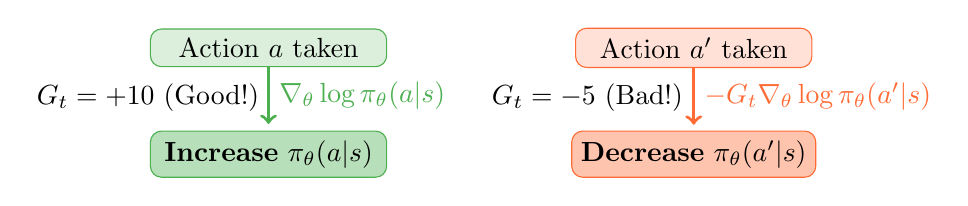
\begin{tikzpicture}[scale=0.9]
                % Good action
                \node[rectangle, draw=drladvantage, fill=drladvantage!20, rounded corners=4pt, minimum width=3cm] (good) at (0,2)
                    {Action $a$ taken};
                \node at (-1.7, 1.3) {$G_t = +10$ (Good!)};

                \draw[->, very thick, drladvantage] (good.south) -- +(0,-0.8) node[midway, right]
                    {$\nabla_\theta \log \pi_\theta(a|s)$};

                \node[rectangle, draw=drladvantage, fill=drladvantage!40, rounded corners=4pt, minimum width=3cm] (goodupdate) at (0,0.5)
                    {\textbf{Increase} $\pi_\theta(a|s)$};

                % Bad action
                \node[rectangle, draw=drlaccent, fill=drlaccent!20, rounded corners=4pt, minimum width=3cm] (bad) at (6,2)
                    {Action $a'$ taken};
                \node at (4.5, 1.3) {$G_t = -5$ (Bad!)};

                \draw[->, very thick, drlaccent] (bad.south) -- +(0,-0.8) node[midway, right]
                    {$-G_t \nabla_\theta \log \pi_\theta(a'|s)$};

                \node[rectangle, draw=drlaccent, fill=drlaccent!40, rounded corners=4pt, minimum width=3cm] (badupdate) at (6,0.5)
                    {\textbf{Decrease} $\pi_\theta(a'|s)$};
            \end{tikzpicture}
        \end{center}
    \end{block}
\end{frame}

\subsection{REINFORCE Algorithm}

\begin{frame}
    \frametitle{The REINFORCE Algorithm}

    \begin{block}<1->{Monte Carlo Policy Gradient}
        REINFORCE is the simplest policy gradient algorithm:
        \begin{itemize}
            \item<2-> Use complete episodes (Monte Carlo)
            \item<3-> Estimate gradient from sampled trajectories
            \item<4-> Update policy in direction of higher expected return
        \end{itemize}
    \end{block}

    \begin{block}<5->{The Update Rule}
        For each episode, for each time step $t$:
        \begin{equation*}
            \theta \leftarrow \theta + \alpha G_t \nabla_\theta \log \pi_\theta(a_t|s_t)
        \end{equation*}
        where $G_t = \sum_{k=t}^T \gamma^{k-t} r_k$ is the return from time $t$.
    \end{block}
\end{frame}

\begin{frame}[fragile]
    \frametitle{REINFORCE Algorithm}

    \begin{algorithm}[H]
        \caption{REINFORCE (Monte Carlo Policy Gradient)}
        \begin{algorithmic}[1]
            \State Initialize policy parameters $\theta$ randomly
            \For{episode $= 1, 2, \ldots$}
                \State Generate episode $s_0, a_0, r_0, s_1, a_1, r_1, \ldots, s_T$ following $\pi_\theta$
                \For{$t = 0$ to $T-1$}
                    \State Compute return: $G_t \leftarrow \sum_{k=t}^{T-1} \gamma^{k-t} r_k$
                    \State Update: $\theta \leftarrow \theta + \alpha \gamma^t G_t \nabla_\theta \log \pi_\theta(a_t|s_t)$
                \EndFor
            \EndFor
        \end{algorithmic}
    \end{algorithm}

    \begin{block}<2->{Key Properties}
        \begin{itemize}
            \item<2-> \textcolor{drladvantage}{\textbf{Unbiased}}: Gradient estimate is correct in expectation
            \item<3-> \textcolor{drlaccent}{\textbf{High Variance}}: Returns can vary significantly
        \end{itemize}
    \end{block}
\end{frame}

\begin{frame}
    \frametitle{REINFORCE Example: CartPole}

    \begin{center}
        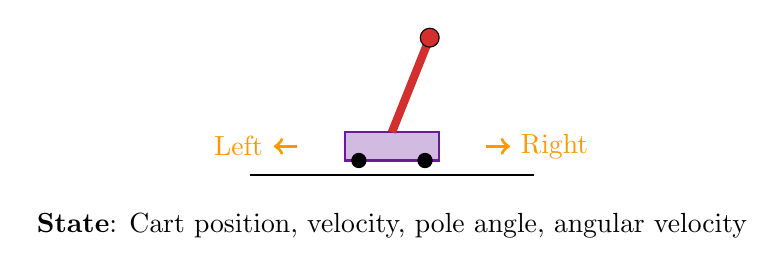
\begin{tikzpicture}[scale=0.6]
            % Cart
            \draw[fill=drlmain!30, draw=drlmain, thick] (-1,-0.3) rectangle (1,0.3);
            \draw[fill=black] (-0.7,-0.3) circle (0.15);
            \draw[fill=black] (0.7,-0.3) circle (0.15);

            % Pole
            \draw[line width=3pt, drlpolicy] (0,0.3) -- (0.8,2.3);
            \draw[fill=drlpolicy] (0.8,2.3) circle (0.2);

            % Ground
            \draw[thick] (-3,-0.6) -- (3,-0.6);

            % Action arrows
            \draw[->, very thick, drlgradient] (-2,0) -- (-2.5,0) node[left] {Left};
            \draw[->, very thick, drlgradient] (2,0) -- (2.5,0) node[right] {Right};

            \node[below] at (0,-1.2) {\textbf{State}: Cart position, velocity, pole angle, angular velocity};
        \end{tikzpicture}
    \end{center}

    \begin{columns}
        \begin{column}{0.45\textwidth}
            \begin{block}<2->{Policy Network}
                \begin{itemize}
                    \item<2-> \textbf{Input}: 4-dimensional state vector
                    \item<3-> \textbf{Hidden Layers}: 2 layers with ReLU activation
                    \item<4-> \textbf{Output}: 2 action probabilities (left/right) with softmax
                \end{itemize}
            \end{block}
        \end{column}

        \begin{column}{0.55\textwidth}
            \begin{block}<5->{Training with REINFORCE}
                \begin{itemize}
                    \item<5-> Episode ends when pole falls or cart leaves track
                    \item<6-> $G_t$: Total remaining reward (episode length)
                    \item<7-> Update increases probability of actions that led to longer episodes
                \end{itemize}
            \end{block}
        \end{column}
    \end{columns}

\end{frame}

\subsection{The Variance Problem}

\begin{frame}
    \frametitle{The High Variance Problem}

    \begin{block}<1->{The Challenge}
        REINFORCE has \textcolor{drlaccent}{\textbf{very high variance}} in gradient estimates!
    \end{block}

    \begin{columns}
        \begin{column}{0.5\textwidth}
            \begin{block}<2->{Why High Variance?}
                \begin{itemize}
                    \item<2-> Returns $G_t$ vary a lot
                    \item<4-> Stochastic environments
                    \item<5-> Long episodes compound uncertainty
                \end{itemize}
            \end{block}
        \end{column}
        \begin{column}{0.5\textwidth}
            \begin{center}
                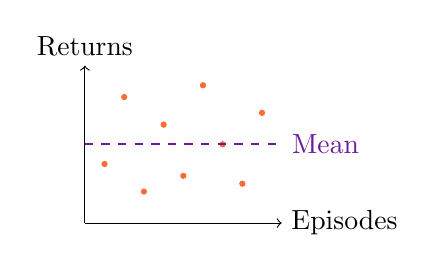
\begin{tikzpicture}[scale=0.5]
                    % High variance illustration
                    \draw[->] (0,0) -- (5,0) node[right] {Episodes};
                    \draw[->] (0,0) -- (0,4) node[above] {Returns};

                    % Noisy returns
                    \foreach \x/\y in {0.5/1.5, 1/3.2, 1.5/0.8, 2/2.5, 2.5/1.2, 3/3.5, 3.5/2.0, 4/1.0, 4.5/2.8} {
                        \fill[drlaccent] (\x,\y) circle (0.08);
                    }

                    % Mean line
                    \draw[dashed, thick, drlmain] (0,2) -- (5,2) node[right] {Mean};

                    % \node[below] at (2.5,-0.5) {\textcolor{drlaccent}{High Variance!}};
                \end{tikzpicture}
            \end{center}
        \end{column}
    \end{columns}
    \begin{block}<6->{Consequences}
        \begin{itemize}
            \item<6-> Slow learning (need many samples)
            \item<7-> Unstable training
            \item<8-> Difficulty finding optimal policy
        \end{itemize}
    \end{block}
\end{frame}

\begin{frame}
    \frametitle{Reducing Variance: The Baseline}

    \begin{block}<1->{Key Idea}
        Subtract a \textcolor{drlvalue}{\textbf{baseline}} $b(s_t)$ from the return:
        \begin{equation*}
            \nabla_\theta J(\theta) = \mathbb{E}_{\pi_\theta} \left[ (G_t - b(s_t)) \nabla_\theta \log \pi_\theta(a_t|s_t) \right]
        \end{equation*}
    \end{block}

    \begin{block}<2->{Why Does This Help?}
        \begin{itemize}
            \item<3-> Baseline shifts returns but \textcolor{drladvantage}{\textbf{doesn't change expectation}} (unbiased!)
            \item<4-> \textcolor{drlvalue}{\textbf{Reduces variance}} by centering returns around zero
            \item<5-> Tells us if action was \textcolor{drladvantage}{\textbf{better or worse than expected}}
        \end{itemize}
    \end{block}
\end{frame}

\begin{frame}
    \frametitle{Reducing Variance: The Baseline}

    \begin{block}{Key Idea}
        Subtract a \textcolor{drlvalue}{\textbf{baseline}} $b(s_t)$ from the return:
        \begin{equation*}
            \nabla_\theta J(\theta) = \mathbb{E}_{\pi_\theta} \left[ (G_t - b(s_t)) \nabla_\theta \log \pi_\theta(a_t|s_t) \right]
        \end{equation*}
    \end{block}

    \begin{block}<1->{Common Choice}
        Use the value function as baseline: $b(s_t) = V(s_t)$
        \begin{equation*}
            \text{Advantage: } A(s_t, a_t) = G_t - V(s_t)
        \end{equation*}
    \end{block}
\end{frame}

\begin{frame}
    \frametitle{Understanding the Advantage Function}

    \begin{block}<1->{What is the Advantage?}
        \begin{equation*}
            A(s,a) = Q(s,a) - V(s)
        \end{equation*}
        \textcolor{drladvantage}{\textbf{How much better is action $a$ compared to the average action?}}
    \end{block}

    \begin{center}
        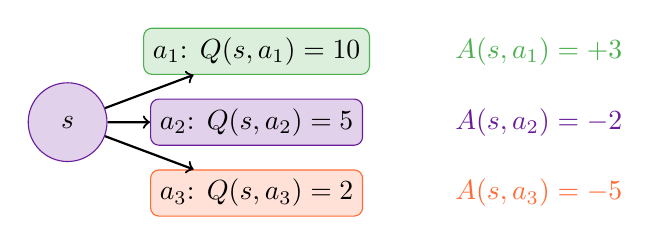
\begin{tikzpicture}[scale=0.6]
            % State
            \node[circle, draw=drlmain, fill=drlmain!20, minimum size=1cm] (s) at (0,2) {$s$};

            % Actions
            \node[rectangle, draw=drladvantage, fill=drladvantage!20, rounded corners=3pt] (a1) at (4,3.5)
                {$a_1$: $Q(s,a_1) = 10$};
            \node[rectangle, draw=drlmain, fill=drlmain!20, rounded corners=3pt] (a2) at (4,2)
                {$a_2$: $Q(s,a_2) = 5$};
            \node[rectangle, draw=drlaccent, fill=drlaccent!20, rounded corners=3pt] (a3) at (4,0.5)
                {$a_3$: $Q(s,a_3) = 2$};

            \draw[->, thick] (s) -- (a1);
            \draw[->, thick] (s) -- (a2);
            \draw[->, thick] (s) -- (a3);

            % Value function
            \node[right] at (8,3.5) {\textcolor{drladvantage}{$A(s,a_1) = +3$}};
            \node[right] at (8,2) {\textcolor{drlmain}{$A(s,a_2) = -2$}};
            \node[right] at (8,0.5) {\textcolor{drlaccent}{$A(s,a_3) = -5$}};
        \end{tikzpicture}
    \end{center}

    \begin{block}<2->{Intuition}
        \begin{itemize}
            \item<2-> $A > 0$: Action is \textcolor{drladvantage}{\textbf{better}} than average $\rightarrow$ increase probability
            \item<3-> $A < 0$: Action is \textcolor{drlaccent}{\textbf{worse}} than average $\rightarrow$ decrease probability
        \end{itemize}
    \end{block}
\end{frame}

% Section: Actor-Critic Methods
\section{Actor-Critic Methods}

\subsection{Combining Policy and Value}

\begin{frame}
    \frametitle{The Actor-Critic Architecture}

    \begin{block}<1->{Two Networks Working Together}
        \begin{itemize}
            \item<2-> \textcolor{drlactor}{\textbf{Actor}}: Policy network $\pi_\theta(a|s)$ (chooses actions)
            \item<3-> \textcolor{drlcritic}{\textbf{Critic}}: Value network $V_\phi(s)$ (evaluates states)
        \end{itemize}
    \end{block}

    \begin{center}
        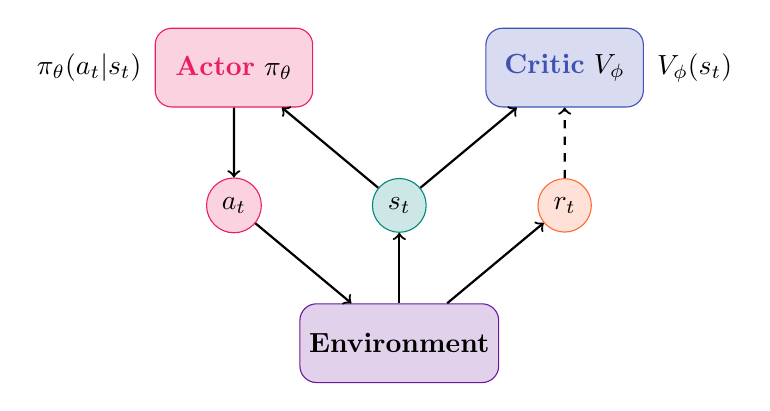
\begin{tikzpicture}[scale=0.7]
            % Environment
            \node[rectangle, draw=drlmain, fill=drlmain!20, rounded corners=6pt, minimum width=2.5cm, minimum height=1cm] (env) at (0,0)
                {\textbf{Environment}};

            % State
            \node[circle, draw=drlsecondary, fill=drlsecondary!20] (state) at (0,2.5) {$s_t$};
            \draw[->, thick] (env) -- (state);

            % Actor
            \node[rectangle, draw=drlactor, fill=drlactor!20, rounded corners=6pt, minimum width=2cm, minimum height=1cm] (actor) at (-3,5)
                {\textcolor{drlactor}{\textbf{Actor}} $\pi_\theta$};
            \draw[->, thick] (state) -- (actor);

            % Critic
            \node[rectangle, draw=drlcritic, fill=drlcritic!20, rounded corners=6pt, minimum width=2cm, minimum height=1cm] (critic) at (3,5)
                {\textcolor{drlcritic}{\textbf{Critic}} $V_\phi$};
            \draw[->, thick] (state) -- (critic);

            % Action
            \node[circle, draw=drlactor, fill=drlactor!20] (action) at (-3,2.5) {$a_t$};
            \draw[->, thick] (actor) -- (action);
            \draw[->, thick] (action) -- (env);

            % Value
            \node[right] at (4.5,5) {$V_\phi(s_t)$};

            % Policy
            \node[left] at (-4.5,5) {$\pi_\theta(a_t|s_t)$};

            % Reward
            \node[circle, draw=drlaccent, fill=drlaccent!20] (reward) at (3,2.5) {$r_t$};
            \draw[->, thick] (env) -- (reward);
            \draw[->, thick, dashed] (reward) -- (critic);
        \end{tikzpicture}
    \end{center}
\end{frame}

\begin{frame}
    \frametitle{Why Actor-Critic?}

    \begin{block}<1->{Advantages Over Pure Policy Gradient}
        \begin{enumerate}
            \item<2-> \textcolor{drladvantage}{\textbf{Lower Variance}}: Use value function instead of Monte Carlo returns
            \item<3-> \textcolor{drlsecondary}{\textbf{Online Learning}}: Can learn from incomplete episodes
            \item<4-> \textcolor{drlmain}{\textbf{More Stable}}: Critic provides baseline for actor
            \item<5-> \textcolor{drlneural}{\textbf{Better Credit Assignment}}: TD learning helps attribute rewards
        \end{enumerate}
    \end{block}

    \begin{block}<6->{The Trade-off}
        \begin{itemize}
            \item<7-> \textcolor{drlaccent}{\textbf{More complex}}: Two networks to train
            \item<8-> \textcolor{drlaccent}{\textbf{Bias introduced}}: Value function is approximate
            \item<9-> But: \textcolor{drladvantage}{\textbf{Usually worth it!}} Much faster learning
        \end{itemize}
    \end{block}
\end{frame}

\subsection{Advantage Actor-Critic (A2C)}

\begin{frame}
    \frametitle{The A2C Algorithm}

    \begin{block}<1->{Advantage Actor-Critic (A2C)}
        Combines policy gradient with learned value function baseline
    \end{block}

    \begin{block}<2->{Key Components}
        \begin{enumerate}
            \item<3-> \textcolor{drlactor}{\textbf{Actor Update}}:
                \begin{equation*}
                    \theta \leftarrow \theta + \alpha_\theta A(s_t, a_t) \nabla_\theta \log \pi_\theta(a_t|s_t)
                \end{equation*}
            \item<4-> \textcolor{drlcritic}{\textbf{Critic Update}}:
                \begin{equation*}
                    \phi \leftarrow \phi + \alpha_\phi A(s_t, a_t) \nabla_\phi V_\phi(s_t)
                \end{equation*}
            \item<5-> \textcolor{drladvantage}{\textbf{Advantage Estimate}}:
                \begin{equation*}
                    A(s_t, a_t) \approx r_t + \gamma V_\phi(s_{t+1}) - V_\phi(s_t)
                \end{equation*}
        \end{enumerate}
    \end{block}
\end{frame}

\begin{frame}
    \frametitle{Understanding the Advantage Estimate}

    \begin{block}<1->{TD Error as Advantage}
        Instead of using Monte Carlo returns $G_t$, use TD error:
        \begin{equation*}
            A(s_t, a_t) \approx \delta_t = r_t + \gamma V_\phi(s_{t+1}) - V_\phi(s_t)
        \end{equation*}
    \end{block}

    \begin{block}<2->{Why This Works}
        \begin{itemize}
            \item<3-> \textcolor{drlvalue}{$V_\phi(s_t)$}: Expected return from state $s_t$
            \item<4-> \textcolor{drlaccent}{$r_t + \gamma V_\phi(s_{t+1})$}: Actual reward + expected future value
            \item<5-> \textcolor{drladvantage}{$\delta_t$}: How much better/worse than expected?
        \end{itemize}
    \end{block}
\end{frame}

\begin{frame}[fragile]
    \begin{algorithm}[H]
        \caption{Advantage Actor-Critic (A2C)}
        \begin{algorithmic}[1]
            \State Initialize actor $\pi_\theta$ and critic $V_\phi$ with random weights
            \For{episode $= 1, 2, \ldots$}
                \State Initialize $s_0$
                \For{$t = 0, 1, 2, \ldots$}
                    \State Sample action: $a_t \sim \pi_\theta(\cdot|s_t)$
                    \State Execute $a_t$, observe $r_t, s_{t+1}$
                    \State Compute TD error: $\delta_t = r_t + \gamma V_\phi(s_{t+1}) - V_\phi(s_t)$
                    \State \textcolor{drlcritic}{\textbf{Update Critic}}: $\phi \leftarrow \phi + \alpha_\phi \delta_t \nabla_\phi V_\phi(s_t)$
                    \State \textcolor{drlactor}{\textbf{Update Actor}}: $\theta \leftarrow \theta + \alpha_\theta \delta_t \nabla_\theta \log \pi_\theta(a_t|s_t)$
                    \If{$s_{t+1}$ is terminal}
                        \State \textbf{break}
                    \EndIf
                \EndFor
            \EndFor
        \end{algorithmic}
    \end{algorithm}
\end{frame}

\begin{frame}
    \frametitle{A2C: Step-by-Step Visualization}

    \begin{center}
        \begin{tikzpicture}[scale=0.75]
            % Time steps
            \foreach \x/\step in {0/t, 3/t+1, 6/t+2} {
                \node[circle, draw=drlmain, fill=drlmain!20] (s\step) at (\x,3) {$s_{\step}$};
                \node[circle, draw=drlactor, fill=drlactor!20] (a\step) at (\x,1) {$a_{\step}$};
                \draw[->, thick] (s\step) -- (a\step);
            }

            % Rewards
            \node[circle, draw=drlaccent, fill=drlaccent!20] (r1) at (1.25,-0.5) {$r_t$};
            \node[circle, draw=drlaccent, fill=drlaccent!20] (r2) at (4.75,-0.5) {$r_{t+1}$};

            % Transitions
            \draw[->, thick] (at) -- (r1);
            \draw[->, thick] (r1) -- (st+1);
            \draw[->, thick] (at+1) -- (r2);
            \draw[->, thick] (r2) -- (st+2);

            % Value estimates
            \only<2->{
                \node[above=5pt of st, drlcritic] {$V_\phi(s_t)$};
                \node[above=5pt of st+1, drlcritic] {$V_\phi(s_{t+1})$};
            }

            % TD error computation
            \only<3->{
                \node[rectangle, draw=drladvantage, fill=drladvantage!20, rounded corners=3pt, minimum width=5cm] at (3.5,-2)
                    {$\delta_t = r_t + \gamma V_\phi(s_{t+1}) - V_\phi(s_t)$};
            }

            % Updates
            \only<4->{
                \draw[->, very thick, drlcritic, dashed] (3.5,-2.8) -- (0,-3.5)
                    node[below, text width=2.5cm, align=center] {\small Critic Update};
                \draw[->, very thick, drlactor, dashed] (3.5,-2.8) -- (7,-3.5)
                    node[below, text width=2.5cm, align=center] {\small Actor Update};
            }
        \end{tikzpicture}
    \end{center}
\end{frame}

\subsection{Network Architecture}

\begin{frame}
    \frametitle{A2C Network Architecture}

    \begin{center}
        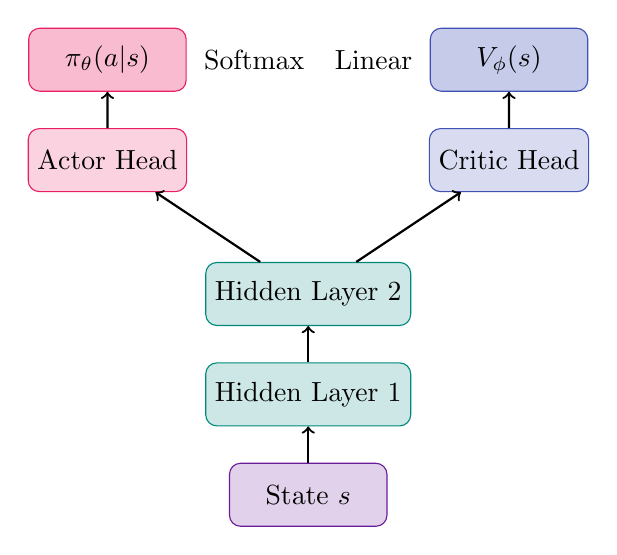
\begin{tikzpicture}[scale=0.85]
            % Input
            \node[rectangle, draw=drlmain, fill=drlmain!20, rounded corners=4pt, minimum width=2cm, minimum height=0.8cm] (input) at (0,0)
                {State $s$};

            % Shared layers
            \node[rectangle, draw=drlsecondary, fill=drlsecondary!20, rounded corners=4pt, minimum width=2.5cm, minimum height=0.8cm] (hidden1) at (0,1.5)
                {Hidden Layer 1};
            \node[rectangle, draw=drlsecondary, fill=drlsecondary!20, rounded corners=4pt, minimum width=2.5cm, minimum height=0.8cm] (hidden2) at (0,3)
                {Hidden Layer 2};

            \draw[->, thick] (input) -- (hidden1);
            \draw[->, thick] (hidden1) -- (hidden2);

            % Actor head
            \node[rectangle, draw=drlactor, fill=drlactor!20, rounded corners=4pt, minimum width=2cm, minimum height=0.8cm] (actor) at (-3,5)
                {Actor Head};
            \node[rectangle, draw=drlactor, fill=drlactor!30, rounded corners=4pt, minimum width=2cm, minimum height=0.8cm] (policy) at (-3,6.5)
                {$\pi_\theta(a|s)$};

            \draw[->, thick] (hidden2) -- (actor);
            \draw[->, thick] (actor) -- (policy);
            \node[right] at (-1.7,6.5) {Softmax};

            % Critic head
            \node[rectangle, draw=drlcritic, fill=drlcritic!20, rounded corners=4pt, minimum width=2cm, minimum height=0.8cm] (critic) at (3,5)
                {Critic Head};
            \node[rectangle, draw=drlcritic, fill=drlcritic!30, rounded corners=4pt, minimum width=2cm, minimum height=0.8cm] (value) at (3,6.5)
                {$V_\phi(s)$};

            \draw[->, thick] (hidden2) -- (critic);
            \draw[->, thick] (critic) -- (value);
            \node[left] at (1.7,6.5) {Linear};
        \end{tikzpicture}
    \end{center}

\end{frame}

\begin{frame}
    \frametitle{Why Share Layers?}

    \begin{columns}
        \begin{column}{0.5\textwidth}
            \begin{block}<1->{Separate Networks}
                \begin{itemize}
                    \item<2-> Independent feature learning
                    \item<3-> More parameters
                    \item<4-> Slower training
                    \item<5-> May learn redundant features
                \end{itemize}
            \end{block}
        \end{column}
        \begin{column}{0.5\textwidth}
            \begin{block}<6->{Shared Layers}
                \begin{itemize}
                    \item<7-> \textcolor{drladvantage}{\textbf{Shared representations}}
                    \item<8-> \textcolor{drladvantage}{\textbf{Fewer parameters}}
                    \item<9-> \textcolor{drladvantage}{\textbf{Faster training}}
                    \item<10-> \textcolor{drladvantage}{\textbf{Better generalization}}
                \end{itemize}
            \end{block}
        \end{column}
    \end{columns}

    \vspace{1em}

    \begin{block}<11->{The Intuition}
        \textcolor{drlmain}{\textbf{Both actor and critic need to understand the state!}} \\
        Share the feature extraction, specialize at the output.
    \end{block}
\end{frame}

\subsection{Training Details}

\begin{frame}
    \frametitle{From Algorithm to Implementation}

    \begin{block}<1->{Recall: A2C Update Rules}
        We've seen how A2C works algorithmically:
        \begin{itemize}
            \item<2-> \textcolor{drlactor}{\textbf{Actor}}: $\theta \leftarrow \theta + \alpha_\theta A_t \nabla_\theta \log \pi_\theta(a_t|s_t)$
            \item<3-> \textcolor{drlcritic}{\textbf{Critic}}: $\phi \leftarrow \phi + \alpha_\phi \delta_t \nabla_\phi V_\phi(s_t)$
        \end{itemize}
    \end{block}

    \begin{block}<4->{The Implementation Challenge}
        \begin{center}
            \textcolor{drlaccent}{\textbf{How do we actually train neural networks with these updates?}}
        \end{center}
    \end{block}

    \begin{block}<5->{The Solution: Loss Functions}
        \begin{itemize}
            \item<6-> Modern deep learning frameworks expect \textcolor{drlneural}{\textbf{loss functions to minimize}}
            \item<7-> They automatically compute gradients via backpropagation
            \item<8-> We need to \textcolor{drlmain}{\textbf{reformulate our updates as losses}}
        \end{itemize}
    \end{block}
\end{frame}

\begin{frame}
    \frametitle{Converting Updates to Loss Functions}

    \begin{block}<1->{The Key Idea}
        \textcolor{drlmain}{\textbf{Gradient descent on loss $L$}} $\equiv$ \textcolor{drladvantage}{\textbf{Gradient ascent on objective $J$}}
        \begin{equation*}
            \theta \leftarrow \theta - \alpha \nabla_\theta L(\theta) \quad \Leftrightarrow \quad \theta \leftarrow \theta + \alpha \nabla_\theta J(\theta)
        \end{equation*}
    \end{block}

    \begin{block}<2->{Therefore: $L = -J$}
        If we want to maximize $J$, we minimize $L = -J$
    \end{block}

    \begin{block}<3->{Actor: From Update Rule to Loss}
        \begin{itemize}
            \item<4-> \textbf{Update rule}: $\theta \leftarrow \theta + \alpha \textcolor{drladvantage}{A_t \nabla_\theta \log \pi_\theta(a_t|s_t)}$
            \item<5-> \textbf{Gradient we want}: $\nabla_\theta J = A_t \nabla_\theta \log \pi_\theta(a_t|s_t)$
            \item<6-> \textbf{Loss function}: $L_\text{actor} = -A_t \log \pi_\theta(a_t|s_t)$
            \item<7-> Check: $\nabla_\theta L_\text{actor} = -A_t \nabla_\theta \log \pi_\theta(a_t|s_t)$ \textcolor{drladvantage}{(correct!)}
        \end{itemize}
    \end{block}
\end{frame}

\begin{frame}
    \frametitle{Converting Updates to Loss Functions (cont.)}

    \begin{block}<1->{Critic: From Update Rule to Loss}
        \begin{itemize}
            \item<2-> \textbf{Update rule}: $\phi \leftarrow \phi + \alpha \textcolor{drlcritic}{\delta_t \nabla_\phi V_\phi(s_t)}$
            \item<3-> where $\delta_t = r_t + \gamma V_\phi(s_{t+1}) - V_\phi(s_t)$ is the TD error
            \item<4-> \textbf{But wait!} This is actually minimizing squared error:
            \begin{equation*}
                \nabla_\phi \frac{1}{2}(r_t + \gamma V_\phi(s_{t+1}) - V_\phi(s_t))^2 = -\delta_t \nabla_\phi V_\phi(s_t)
            \end{equation*}
            \item<5-> \textbf{Loss function}: $L_\text{critic} = \frac{1}{2}\delta_t^2 = \frac{1}{2}(r_t + \gamma V_\phi(s_{t+1}) - V_\phi(s_t))^2$
        \end{itemize}
    \end{block}

    \begin{block}<6->{Key Insight}
        \begin{itemize}
            \item<7-> \textcolor{drlactor}{\textbf{Actor}}: Maximize objective $\rightarrow$ negate it to get loss
            \item<8-> \textcolor{drlcritic}{\textbf{Critic}}: Already minimizing error $\rightarrow$ use squared error directly
        \end{itemize}
    \end{block}
\end{frame}

\begin{frame}
    \frametitle{Loss Functions in A2C}

    \begin{block}<1->{Actor Loss (Policy Gradient)}
        \begin{equation*}
            L_\text{actor} = -\log \pi_\theta(a_t|s_t) \cdot A_t
        \end{equation*}
    \end{block}

    \begin{block}<2->{Critic Loss (Value Function)}
        \begin{equation*}
            L_\text{critic} = (r_t + \gamma V_\phi(s_{t+1}) - V_\phi(s_t))^2
        \end{equation*}
    \end{block}
    \end{frame}

\begin{frame}
    \frametitle{The Problem: Premature Convergence}

    \begin{block}<1->{What Can Go Wrong?}
        Policy gradient methods can converge to a deterministic policy too quickly!
    \end{block}

    \begin{columns}
        \begin{column}{0.5\textwidth}
            \begin{block}<2->{Early Training}
                \begin{center}
                    \textcolor{drladvantage}{\textbf{Exploratory}}
                    \end{center}
                \begin{itemize}
                    \item<3-> Policy tries different actions
                    \item<4-> Discovers better strategies
                    \item<5-> Learns from diverse experience
                \end{itemize}
            \end{block}
        \end{column}
        \begin{column}{0.5\textwidth}
            \begin{block}<6->{Too Fast Convergence}
                \begin{center}
                    \textcolor{drlaccent}{\textbf{Stuck!}}
                    \end{center}
                \begin{itemize}
                    \item<7-> Policy becomes deterministic
                    \item<8-> Stops exploring alternatives
                    \item<9-> Gets stuck in local optimum
                \end{itemize}
            \end{block}
        \end{column}
    \end{columns}

    \begin{block}<10->{The Solution}
        \textcolor{drlmain}{\textbf{Add entropy bonus to encourage exploration!}}
    \end{block}
\end{frame}

\begin{frame}
    \frametitle{Entropy: Measuring Policy Randomness}

    \begin{block}<1->{Entropy Definition}
        Entropy measures the \textcolor{drlmain}{\textbf{randomness}} or \textcolor{drlmain}{\textbf{uncertainty}} in the policy:
        \begin{equation*}
            H(\pi_\theta) = -\sum_a \pi_\theta(a|s) \log \pi_\theta(a|s)
        \end{equation*}
    \end{block}

    \begin{block}<2->{Intuition}
        \begin{itemize}
            \item<3-> \textcolor{drladvantage}{\textbf{High entropy}}: Policy is uniform, explores many actions
            \item<4-> \textcolor{drlaccent}{\textbf{Low entropy}}: Policy is deterministic, picks one action
        \end{itemize}
    \end{block}
\end{frame}

\begin{frame}
    \frametitle{Entropy: Measuring Policy Randomness}

    \begin{block}{Entropy Definition}
        Entropy measures the \textcolor{drlmain}{\textbf{randomness}} or \textcolor{drlmain}{\textbf{uncertainty}} in the policy:
        \begin{equation*}
            H(\pi_\theta) = -\sum_a \pi_\theta(a|s) \log \pi_\theta(a|s)
        \end{equation*}
    \end{block}

    \begin{columns}
        \begin{column}{0.5\textwidth}
            \begin{block}<5->{Low Entropy}
                \begin{itemize}
                    \item<6-> $\pi(a_1|s) = 0.99$
                    \item<6-> $\pi(a_2|s) = 0.01$
                    \item<7-> $H \approx 0.06$
                \end{itemize}
            \end{block}
        \end{column}
        \begin{column}{0.5\textwidth}
            \begin{block}<9->{High Entropy}
                \begin{itemize}
                    \item<10-> $\pi(a_1|s) = 0.5$
                    \item<10-> $\pi(a_2|s) = 0.5$
                    \item<11-> $H = 0.69$
                \end{itemize}
            \end{block}
        \end{column}
    \end{columns}
\end{frame}

\begin{frame}
    \frametitle{Adding Entropy to the Loss Function}

    \begin{block}<1->{The Entropy Bonus}
        We \textcolor{drladvantage}{\textbf{subtract}} entropy from the loss (equivalently, add to reward):
        \begin{equation*}
            L_\text{total} = L_\text{actor} + c_1 L_\text{critic} - c_2 H(\pi_\theta)
        \end{equation*}
        where $c_2 > 0$ is the \textcolor{drlmain}{\textbf{entropy coefficient}} (typically $c_2 = 0.01$)
    \end{block}

    \begin{block}<2->{Why Subtract (Not Add)?}
        \begin{itemize}
            \item<3-> \textcolor{drladvantage}{\textbf{High entropy}} $\rightarrow$ negative term is large (more negative)
            \item<4-> \textcolor{drladvantage}{\textbf{Lower total loss}} $\rightarrow$ encourage this policy
            \item<5-> Effect: \textcolor{drlmain}{\textbf{Rewards exploration!}}
        \end{itemize}
    \end{block}

    \begin{block}<6->{Balancing Act}
        \begin{itemize}
            \item<7-> Too low $c_2$: Policy converges too fast (exploitation)
            \item<8-> Too high $c_2$: Policy stays random forever (too much exploration)
            \item<9-> \textcolor{drlmain}{\textbf{Sweet spot}}: $c_2 = 0.01$ works well in practice
        \end{itemize}
    \end{block}
\end{frame}

\begin{frame}
    \frametitle{Adding Entropy to the Loss Function}

    \begin{block}{The Entropy Bonus}
        We \textcolor{drladvantage}{\textbf{subtract}} entropy from the loss (equivalently, add to reward):
        \begin{equation*}
            L_\text{total} = L_\text{actor} + c_1 L_\text{critic} - c_2 H(\pi_\theta)
        \end{equation*}
        where $c_2 > 0$ is the \textcolor{drlmain}{\textbf{entropy coefficient}} (typically $c_2 = 0.01$)
    \end{block}

    \begin{block}{Balancing Act}
        \begin{itemize}
            \item<2-> Too low $c_2$: Policy converges too fast (exploitation)
            \item<3-> Too high $c_2$: Policy stays random forever (too much exploration)
            \item<4-> \textcolor{drlmain}{\textbf{Sweet spot}}: $c_2 = 0.01$ works well in practice
        \end{itemize}
    \end{block}
\end{frame}

\begin{frame}
    \frametitle{Why Combine Into a Total Loss?}

    \begin{block}<1->{Separate vs. Joint Training}
        We have actor loss, critic loss, and entropy — why combine them?
    \end{block}

    \begin{block}<2->{Reason 1: Shared Network Architecture}
        \begin{itemize}
            \item<3-> In practice, actor and critic often \textcolor{drlmain}{\textbf{share layers}}
            \item<4-> Early layers extract features from states
            \item<5-> Network splits into policy head (actor) and value head (critic)
            \item<6-> \textcolor{drladvantage}{\textbf{Need single loss}} to backpropagate through shared layers
        \end{itemize}
    \end{block}

    \begin{block}<7->{Reason 2: Balancing Objectives}
        \begin{itemize}
            \item<8-> $c_1 L_\text{critic}$: how much to prioritize accurate value estimates
            \item<9-> $c_2 H(\pi_\theta)$: how much to prioritize exploration
            \item<10-> \textcolor{drlmain}{\textbf{Joint optimization}} enables efficient learning
        \end{itemize}
    \end{block}
\end{frame}

\begin{frame}
    \frametitle{Complete A2C Loss Function}

    \begin{block}<1->{All Three Components Together}
        \begin{equation*}
            L_\text{total} = L_\text{actor} + c_1 L_\text{critic} - c_2 H(\pi_\theta)
        \end{equation*}
    \end{block}

    \begin{block}<2->{Breaking It Down}
        \begin{itemize}
            \item<3-> \textcolor{drlactor}{\textbf{Actor loss}}: $L_\text{actor} = -A_t \log \pi_\theta(a_t|s_t)$ \\
                      \small{Maximize advantage-weighted log probabilities}
            \item<4-> \textcolor{drlcritic}{\textbf{Critic loss}}: $L_\text{critic} = \frac{1}{2}\delta_t^2$ \\
                      \small{Minimize TD error (coefficient $c_1 = 0.5$ typical)}
            \item<5-> \textcolor{drladvantage}{\textbf{Entropy bonus}}: $-c_2 H(\pi_\theta)$ \\
                      \small{Encourage exploration (coefficient $c_2 = 0.01$ typical)}
        \end{itemize}
    \end{block}
\end{frame}

\begin{frame}
    \frametitle{A2C Implementation Tips}

    \begin{block}<1->{Hyperparameters}
        \begin{itemize}
            \item<2-> \textbf{Learning rates}: Typically $\alpha_\theta = 10^{-4}$, $\alpha_\phi = 10^{-3}$
            \item<3-> \textbf{Discount factor}: $\gamma = 0.99$ (standard choice)
            \item<4-> \textbf{Entropy coefficient}: $c_2 = 0.01$ (small but important)
            \item<5-> \textbf{Value loss coefficient}: $c_1 = 0.5$
        \end{itemize}
    \end{block}

    \begin{block}<6->{Training Tricks}
        \begin{itemize}
            \item<7-> \textcolor{drladvantage}{\textbf{Normalize advantages}}: Zero mean, unit variance
            \item<8-> \textcolor{drlsecondary}{\textbf{Gradient clipping}}: Prevent exploding gradients
            \item<9-> \textcolor{drlmain}{\textbf{Orthogonal initialization}}: Better than random
            \item<10-> \textcolor{drlneural}{\textbf{Learning rate scheduling}}: Decay over time
        \end{itemize}
    \end{block}
\end{frame}

\subsection{A2C vs A3C}

\begin{frame}
    \frametitle{A2C vs A3C: What's the Difference?}

    \begin{block}<1->{A3C: Asynchronous Advantage Actor-Critic}
        \begin{itemize}
            \item<2-> Multiple actors running in \textcolor{drlaccent}{\textbf{parallel}}
            \item<3-> Each actor interacts with separate environment copy
            \item<4-> Updates happen \textcolor{drlaccent}{\textbf{asynchronously}}
            \item<5-> More exploration, faster training
        \end{itemize}
    \end{block}

    \begin{block}<6->{A2C: Advantage Actor-Critic (Synchronous)}
        \begin{itemize}
            \item<7-> Multiple actors, but updates are \textcolor{drladvantage}{\textbf{synchronized}}
            \item<8-> Wait for all actors before updating
            \item<9-> Simpler implementation
            \item<10-> Better GPU utilization
        \end{itemize}
    \end{block}
\end{frame}

\begin{frame}
    \frametitle{Parallel A2C Architecture}

    \begin{columns}
        \begin{column}{0.55\textwidth}
            \begin{center}
                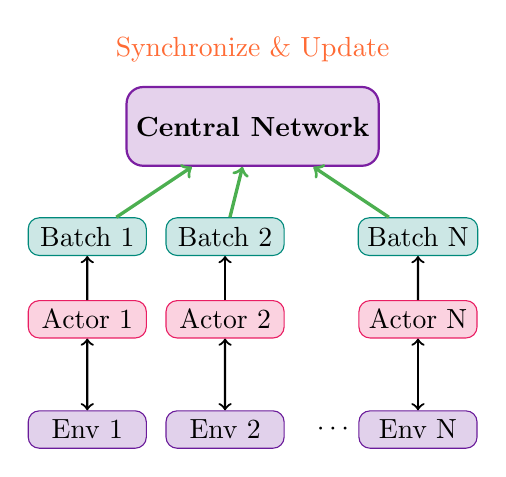
\begin{tikzpicture}[scale=0.7]
                    % Environments
                    \node[rectangle, draw=drlmain, fill=drlmain!20, rounded corners=4pt, minimum width=1.5cm] (env1) at (-4,0) {Env 1};
                    \node[rectangle, draw=drlmain, fill=drlmain!20, rounded corners=4pt, minimum width=1.5cm] (env2) at (-1.5,0) {Env 2};
                    \node at (0.5,0) {$\cdots$};
                    \node[rectangle, draw=drlmain, fill=drlmain!20, rounded corners=4pt, minimum width=1.5cm] (envn) at (2,0) {Env N};

                    % Actors (local copies)
                    \node[rectangle, draw=drlactor, fill=drlactor!20, rounded corners=4pt, minimum width=1.5cm] (actor1) at (-4,2) {Actor 1};
                    \node[rectangle, draw=drlactor, fill=drlactor!20, rounded corners=4pt, minimum width=1.5cm] (actor2) at (-1.5,2) {Actor 2};
                    \node[rectangle, draw=drlactor, fill=drlactor!20, rounded corners=4pt, minimum width=1.5cm] (actorn) at (2,2) {Actor N};

                    \draw[<->, thick] (env1) -- (actor1);
                    \draw[<->, thick] (env2) -- (actor2);
                    \draw[<->, thick] (envn) -- (actorn);

                    % Experience collection
                    \node[rectangle, draw=drlsecondary, fill=drlsecondary!20, rounded corners=4pt, minimum width=1.5cm] (exp1) at (-4,3.5) {Batch 1};
                    \node[rectangle, draw=drlsecondary, fill=drlsecondary!20, rounded corners=4pt, minimum width=1.5cm] (exp2) at (-1.5,3.5) {Batch 2};
                    \node[rectangle, draw=drlsecondary, fill=drlsecondary!20, rounded corners=4pt, minimum width=1.5cm] (expn) at (2,3.5) {Batch N};

                    \draw[->, thick] (actor1) -- (exp1);
                    \draw[->, thick] (actor2) -- (exp2);
                    \draw[->, thick] (actorn) -- (expn);

                    % Central network
                    \node[rectangle, draw=drlneural, fill=drlneural!20, rounded corners=6pt, thick, minimum width=3cm, minimum height=1cm] (central) at (-1,5.5)
                        {\textbf{Central Network}};

                    \draw[->, very thick, drladvantage] (exp1) -- (central);
                    \draw[->, very thick, drladvantage] (exp2) -- (central);
                    \draw[->, very thick, drladvantage] (expn) -- (central);

                    \node[above] at (-1,6.5) {\textcolor{drlaccent}{Synchronize \& Update}};
                \end{tikzpicture}
            \end{center}
        \end{column}
        \begin{column}{0.45\textwidth}
            \begin{block}<2->{Benefits}
                \begin{itemize}
                    \item<2-> \textcolor{drladvantage}{\textbf{More diverse experience}} \\
                              \small{Different actors explore differently}
                    \item<3-> \textcolor{drlsecondary}{\textbf{Faster data collection}} \\
                              \small{N times more experience}
                    \item<4-> \textcolor{drlmain}{\textbf{Better stability}} \\
                              \small{Averaging over multiple environments}
                \end{itemize}
            \end{block}
        \end{column}
    \end{columns}
\end{frame}

% Section: Practical Considerations
\section{Practical Considerations}

\subsection{When to Use Policy Gradients}

\begin{frame}
    \frametitle{Policy Gradients: When to Use?}

    \begin{block}<1->{Good For}
        \begin{itemize}
            \item<2-> \textcolor{drladvantage}{\textbf{Continuous action spaces}}: Robot control, driving
            \item<3-> \textcolor{drladvantage}{\textbf{Stochastic policies}}: Games with mixed strategies
            \item<4-> \textcolor{drladvantage}{\textbf{High-dimensional actions}}: Many simultaneous decisions
            \item<5-> \textcolor{drladvantage}{\textbf{Partially observable environments}}: When state is ambiguous
        \end{itemize}
    \end{block}

    \begin{block}<6->{Challenges}
        \begin{itemize}
            \item<7-> \textcolor{drlaccent}{\textbf{Sample inefficient}}: Need lots of experience
            \item<8-> \textcolor{drlaccent}{\textbf{Sensitive to hyperparameters}}: Learning rates, initialization
            \item<9-> \textcolor{drlaccent}{\textbf{Local optima}}: May not find global optimum
            \item<10-> \textcolor{drlaccent}{\textbf{High variance}}: Even with baselines
        \end{itemize}
    \end{block}
\end{frame}

\begin{frame}
    \frametitle{Comparison with Value-Based Methods}

    \begin{center}
        \begin{tabular}{|l|c|c|}
            \hline
            \textbf{Property} & \textbf{Policy Gradient} & \textbf{Value-Based} \\
            \hline
            Continuous Actions & \textcolor{drladvantage}{\checkmark} & \textcolor{drlaccent}{\texttimes} \\
            Sample Efficiency & \textcolor{drlaccent}{\texttimes} & \textcolor{drladvantage}{\checkmark} \\
            Convergence & \textcolor{drladvantage}{\checkmark} & Approximate \\
            Stochastic Policies & \textcolor{drladvantage}{\checkmark} & \textcolor{drlaccent}{\texttimes} \\
            Stability & Moderate & Can be unstable \\
            Computational Cost & High & Moderate \\
            \hline
        \end{tabular}
    \end{center}

    \vspace{1em}

    \begin{block}<2->{The Best of Both?}
        \textcolor{drlneural}{\textbf{Actor-Critic methods}} combine advantages of both approaches!
    \end{block}
\end{frame}

\subsection{Common Issues and Solutions}

\begin{frame}
    \frametitle{Common Issues in Policy Gradient Training}

    \begin{block}<1->{Problem 1: High Variance}
        \textbf{Symptoms}: Training is unstable, returns fluctuate wildly
        \begin{itemize}
            \item<2-> \textcolor{drladvantage}{Solution}: Use advantage function with baseline
            \item<3-> \textcolor{drladvantage}{Solution}: Normalize advantages
            \item<4-> \textcolor{drladvantage}{Solution}: Use larger batch sizes
        \end{itemize}
    \end{block}

    \begin{block}<5->{Problem 2: Exploding/Vanishing Gradients}
        \textbf{Symptoms}: Network parameters become very large or zero
        \begin{itemize}
            \item<6-> \textcolor{drladvantage}{Solution}: Gradient clipping
            \item<7-> \textcolor{drladvantage}{Solution}: Proper initialization (orthogonal)
            \item<8-> \textcolor{drladvantage}{Solution}: Batch normalization or layer normalization
        \end{itemize}
    \end{block}
\end{frame}

\begin{frame}
    \frametitle{More Common Issues}

    \begin{block}<1->{Problem 3: Poor Exploration}
        \textbf{Symptoms}: Agent gets stuck in suboptimal policy
        \begin{itemize}
            \item<2-> \textcolor{drladvantage}{Solution}: Entropy bonus in loss function
            \item<3-> \textcolor{drladvantage}{Solution}: Action noise or $\epsilon$-greedy exploration
            \item<4-> \textcolor{drladvantage}{Solution}: Curiosity-driven exploration
        \end{itemize}
    \end{block}

    \begin{block}<5->{Problem 4: Policy Collapse}
        \textbf{Symptoms}: Policy becomes deterministic too quickly
        \begin{itemize}
            \item<6-> \textcolor{drladvantage}{Solution}: Increase entropy coefficient
            \item<7-> \textcolor{drladvantage}{Solution}: Lower learning rate
            \item<8-> \textcolor{drladvantage}{Solution}: Trust region methods (PPO, TRPO)
        \end{itemize}
    \end{block}
\end{frame}

\begin{frame}
    \frametitle{Debugging Tips}

    \begin{block}<1->{Start Simple}
        \begin{enumerate}
            \item<2-> Test on simple environments (CartPole, MountainCar)
            \item<3-> Verify network can fit random data
            \item<4-> Check gradient magnitudes (should be $10^{-3}$ to $10^{0}$)
            \item<5-> Visualize policy and value function
        \end{enumerate}
    \end{block}

    \begin{block}<6->{Monitor Key Metrics}
        \begin{itemize}
            \item<7-> \textcolor{drlvalue}{\textbf{Value loss}}: Should decrease steadily
            \item<8-> \textcolor{drlactor}{\textbf{Policy entropy}}: Should stay moderate
            \item<9-> \textcolor{drladvantage}{\textbf{Advantage mean}}: Should be near zero
            \item<10-> \textcolor{drlmain}{\textbf{Episode returns}}: Should increase over time
            \item<11-> \textcolor{drlgradient}{\textbf{Gradient norms}}: Should not explode
        \end{itemize}
    \end{block}
\end{frame}

% Section: Summary
\section{Summary}

\subsection{Key Takeaways}

\begin{frame}
    \frametitle{What We Learned Today}

    \begin{block}<1->{Policy Gradient Methods}
        \begin{itemize}
            \item<2-> Learn policies \textcolor{drlpolicy}{\textbf{directly}} through gradient ascent
            \item<3-> \textcolor{drlmain}{\textbf{Policy Gradient Theorem}}: $\nabla_\theta J(\theta) = \mathbb{E}[G_t \nabla_\theta \log \pi_\theta(a|s)]$
            \item<4-> \textcolor{drlaccent}{\textbf{REINFORCE}}: Monte Carlo policy gradient algorithm
            \item<5-> Use baselines to reduce variance
        \end{itemize}
    \end{block}

    \begin{block}<6->{Actor-Critic Methods}
        \begin{itemize}
            \item<7-> \textcolor{drlactor}{\textbf{Actor}}: Policy network
            \item<8-> \textcolor{drlcritic}{\textbf{Critic}}: Value network
            \item<9-> \textcolor{drladvantage}{\textbf{A2C}}: Synchronous advantage actor-critic
            \item<10-> Lower variance, faster learning than pure policy gradient
        \end{itemize}
    \end{block}
\end{frame}

\begin{frame}
    \frametitle{Recommended Resources}

    \begin{block}{Implementation}
        \begin{itemize}
            \item OpenAI Spinning Up: \texttt{spinningup.openai.com}
            \item Stable Baselines3: Popular implementations
            \item OpenAI Gym: Standard RL environments
        \end{itemize}
    \end{block}
\end{frame}


\end{document}
